\documentclass[11pt]{article}\usepackage[]{graphicx}\usepackage[]{xcolor}
% maxwidth is the original width if it is less than linewidth
% otherwise use linewidth (to make sure the graphics do not exceed the margin)
\makeatletter
\def\maxwidth{ %
  \ifdim\Gin@nat@width>\linewidth
    \linewidth
  \else
    \Gin@nat@width
  \fi
}
\makeatother

\definecolor{fgcolor}{rgb}{0.345, 0.345, 0.345}
\newcommand{\hlnum}[1]{\textcolor[rgb]{0.686,0.059,0.569}{#1}}%
\newcommand{\hlstr}[1]{\textcolor[rgb]{0.192,0.494,0.8}{#1}}%
\newcommand{\hlcom}[1]{\textcolor[rgb]{0.678,0.584,0.686}{\textit{#1}}}%
\newcommand{\hlopt}[1]{\textcolor[rgb]{0,0,0}{#1}}%
\newcommand{\hlstd}[1]{\textcolor[rgb]{0.345,0.345,0.345}{#1}}%
\newcommand{\hlkwa}[1]{\textcolor[rgb]{0.161,0.373,0.58}{\textbf{#1}}}%
\newcommand{\hlkwb}[1]{\textcolor[rgb]{0.69,0.353,0.396}{#1}}%
\newcommand{\hlkwc}[1]{\textcolor[rgb]{0.333,0.667,0.333}{#1}}%
\newcommand{\hlkwd}[1]{\textcolor[rgb]{0.737,0.353,0.396}{\textbf{#1}}}%
\let\hlipl\hlkwb

\usepackage{framed}
\makeatletter
\newenvironment{kframe}{%
 \def\at@end@of@kframe{}%
 \ifinner\ifhmode%
  \def\at@end@of@kframe{\end{minipage}}%
  \begin{minipage}{\columnwidth}%
 \fi\fi%
 \def\FrameCommand##1{\hskip\@totalleftmargin \hskip-\fboxsep
 \colorbox{shadecolor}{##1}\hskip-\fboxsep
     % There is no \\@totalrightmargin, so:
     \hskip-\linewidth \hskip-\@totalleftmargin \hskip\columnwidth}%
 \MakeFramed {\advance\hsize-\width
   \@totalleftmargin\z@ \linewidth\hsize
   \@setminipage}}%
 {\par\unskip\endMakeFramed%
 \at@end@of@kframe}
\makeatother

\definecolor{shadecolor}{rgb}{.97, .97, .97}
\definecolor{messagecolor}{rgb}{0, 0, 0}
\definecolor{warningcolor}{rgb}{1, 0, 1}
\definecolor{errorcolor}{rgb}{1, 0, 0}
\newenvironment{knitrout}{}{} % an empty environment to be redefined in TeX

\usepackage{alltt}

% Packages for graphics & layout
\usepackage{graphicx}
\usepackage{epstopdf}
\usepackage{subcaption}
\usepackage{booktabs}
\usepackage[a4paper,margin=0.5in]{geometry}

% Packages for math
\usepackage{amsmath}
\usepackage{amsfonts}
\usepackage{amssymb}

% Package for bibliography
\usepackage{natbib}
\usepackage{hyperref}

\title{Data Analysis Report}
\author{[Michael V Cumbo]}
\date{\today}
\IfFileExists{upquote.sty}{\usepackage{upquote}}{}
\begin{document}

\maketitle

\begin{abstract}
This document presents a comprehensive analysis of the data pertaining to trade unions.
\end{abstract}

\section{Introduction}
This paper was written in response to the United Auto Workers strike and the SAG-AFTRA strike of 2023. The goal of this paper is to contextualize the state of trade union power in the United States, blending data analysis with a literature review. The findings in this paper also contextualize union power in a select number of nation-states, adding perspective to the modes of influence individual working-class individuals may have within those states.

\section{Methodology}
\subsection*{Libraries Used in Analysis}

Our analysis utilized several R packages, each contributing unique functions essential for data management, manipulation, visualization, and database interaction. Below is a description of each package and its role in our analysis:

\begin{itemize}
    \item \textbf{tidyverse}: An aggregation of several data manipulation packages, \texttt{tidyverse} simplifies many aspects of data analysis. It includes packages like \texttt{ggplot2} for data visualization, \texttt{dplyr} for data manipulation, and \texttt{readr} for data import. Its unified data philosophy makes data science tasks more straightforward and efficient.
    \begin{itemize}
        \item Installation: \texttt{install.packages("tidyverse")}
        \item Documentation: \href{https://www.tidyverse.org/}{tidyverse.org}
    \end{itemize}
    
    \item \textbf{RSQLite}: This package provides a database interface and SQLite driver for R. It allows for seamless integration of SQLite database capabilities within R, enabling the storage, management, and retrieval of large datasets efficiently.
    \begin{itemize}
        \item Installation: \texttt{install.packages("RSQLite")}
        \item Documentation: \href{https://cran.r-project.org/web/packages/RSQLite/index.html}{RSQLite on CRAN}
    \end{itemize}
    
    \item \textbf{DBI}: The \texttt{DBI} package defines a common interface between R and database management systems. It is crucial for establishing database connections and executing database queries.
    \begin{itemize}
        \item Installation: \texttt{install.packages("DBI")}
        \item Documentation: \href{https://cran.r-project.org/web/packages/DBI/index.html}{DBI on CRAN}
    \end{itemize}
    
    \item \textbf{ggplot2}: A part of the \texttt{tidyverse}, \texttt{ggplot2} is a powerful and flexible tool for creating elegant data visualizations in R. It is based on the Grammar of Graphics and allows for building plots iteratively.
    \begin{itemize}
        \item Installation: \texttt{install.packages("ggplot2")}
        \item Documentation: \href{https://ggplot2.tidyverse.org/}{ggplot2.tidyverse.org}
    \end{itemize}
    
    \item \textbf{dplyr}: Also within the \texttt{tidyverse}, \texttt{dplyr} is used for data manipulation. It provides a set of verbs like filter, select, mutate, and summarize, making data manipulation tasks more intuitive and readable.
    \begin{itemize}
        \item Installation: \texttt{install.packages("dplyr")}
        \item Documentation: \href{https://dplyr.tidyverse.org/}{dplyr.tidyverse.org}
    \end{itemize}
    
    \item \textbf{forcats}: This package, part of the \texttt{tidyverse}, is designed for handling categorical variables (factors in R). It provides functions for reordering factor levels, collapsing levels, and changing the display of factor levels.
    \begin{itemize}
        \item Installation: \texttt{install.packages("forcats")}
        \item Documentation: \href{https://forcats.tidyverse.org/}{forcats.tidyverse.org}
    \end{itemize}
    
    \item \textbf{GGally}: An extension of \texttt{ggplot2}, \texttt{GGally} provides additional functions and utilities to enhance the capability of \texttt{ggplot2}, especially for creating complex multi-plot layouts.
    \begin{itemize}
        \item Installation: \texttt{install.packages("GGally")}
        \item Documentation: \href{https://cran.r-project.org/web/packages/GGally/index.html}{GGally on CRAN}
    \end{itemize}
    
    \item \textbf{stringr}: This package, also a part of the \texttt{tidyverse}, simplifies the process of working with strings (text data). It provides consistent and easy-to-use functions for string manipulation.
    \begin{itemize}
        \item Installation: \texttt{install.packages("stringr")}
        \item Documentation: \href{https://stringr.tidyverse.org/}{stringr.tidyverse.org}
    \end{itemize}
\end{itemize}

These libraries collectively provided the comprehensive toolkit necessary for our data analysis, from data manipulation and querying to visualization and string processing.

\subsection{Data Collection}
Data was sourced from the International Labor Organization, OECD datasets, and Harvard datasets.

\subsection{Data Preparation}
[Explain any preprocessing steps like cleaning, normalization, or transformations.]

\section{Discussion}
Discuss the implications of your findings, potential limitations of your analysis, and suggestions for future research.




\begin{figure}[h]
\centering
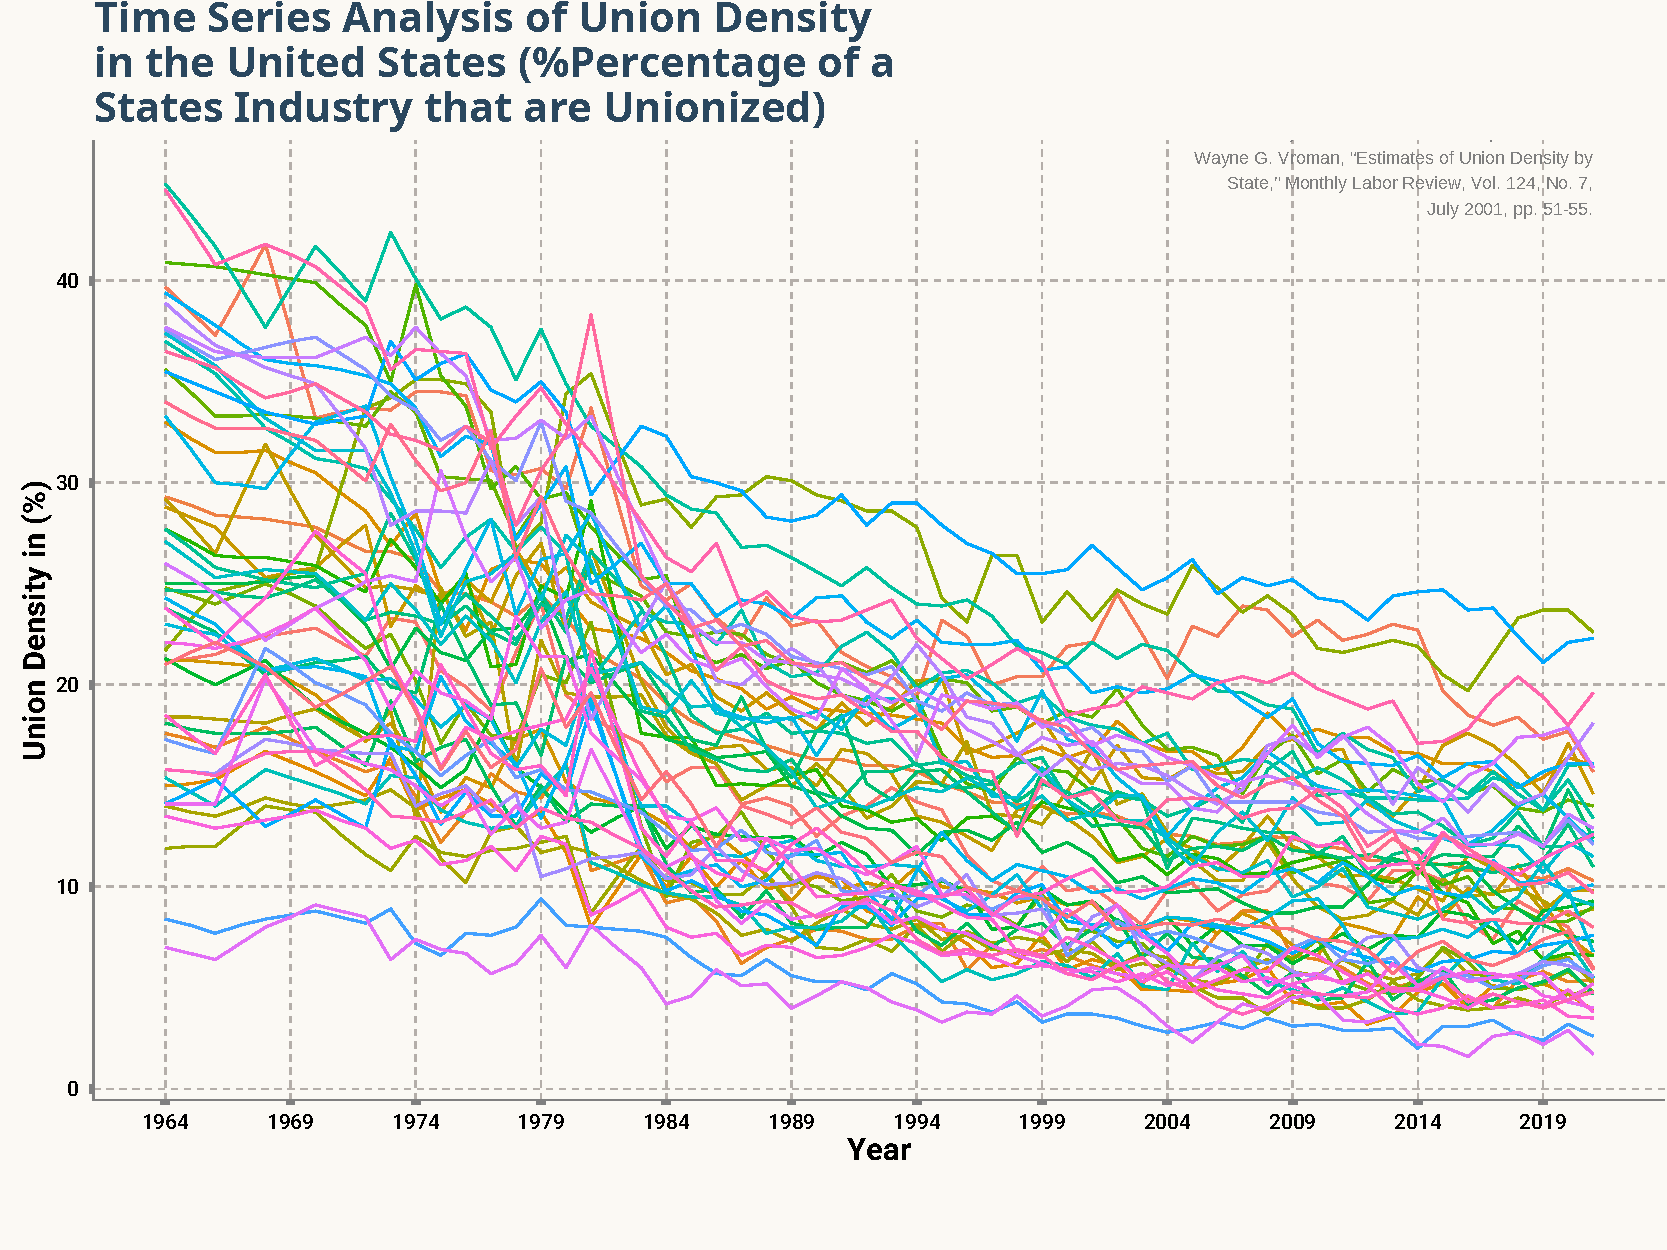
\includegraphics[width=.7\textwidth]{~/Lab2/graphs/plot_10.pdf}
\caption{[Detailed caption for Figure 1]}
\label{fig:1.1}
\end{figure}

\begin{figure}[h]
\centering
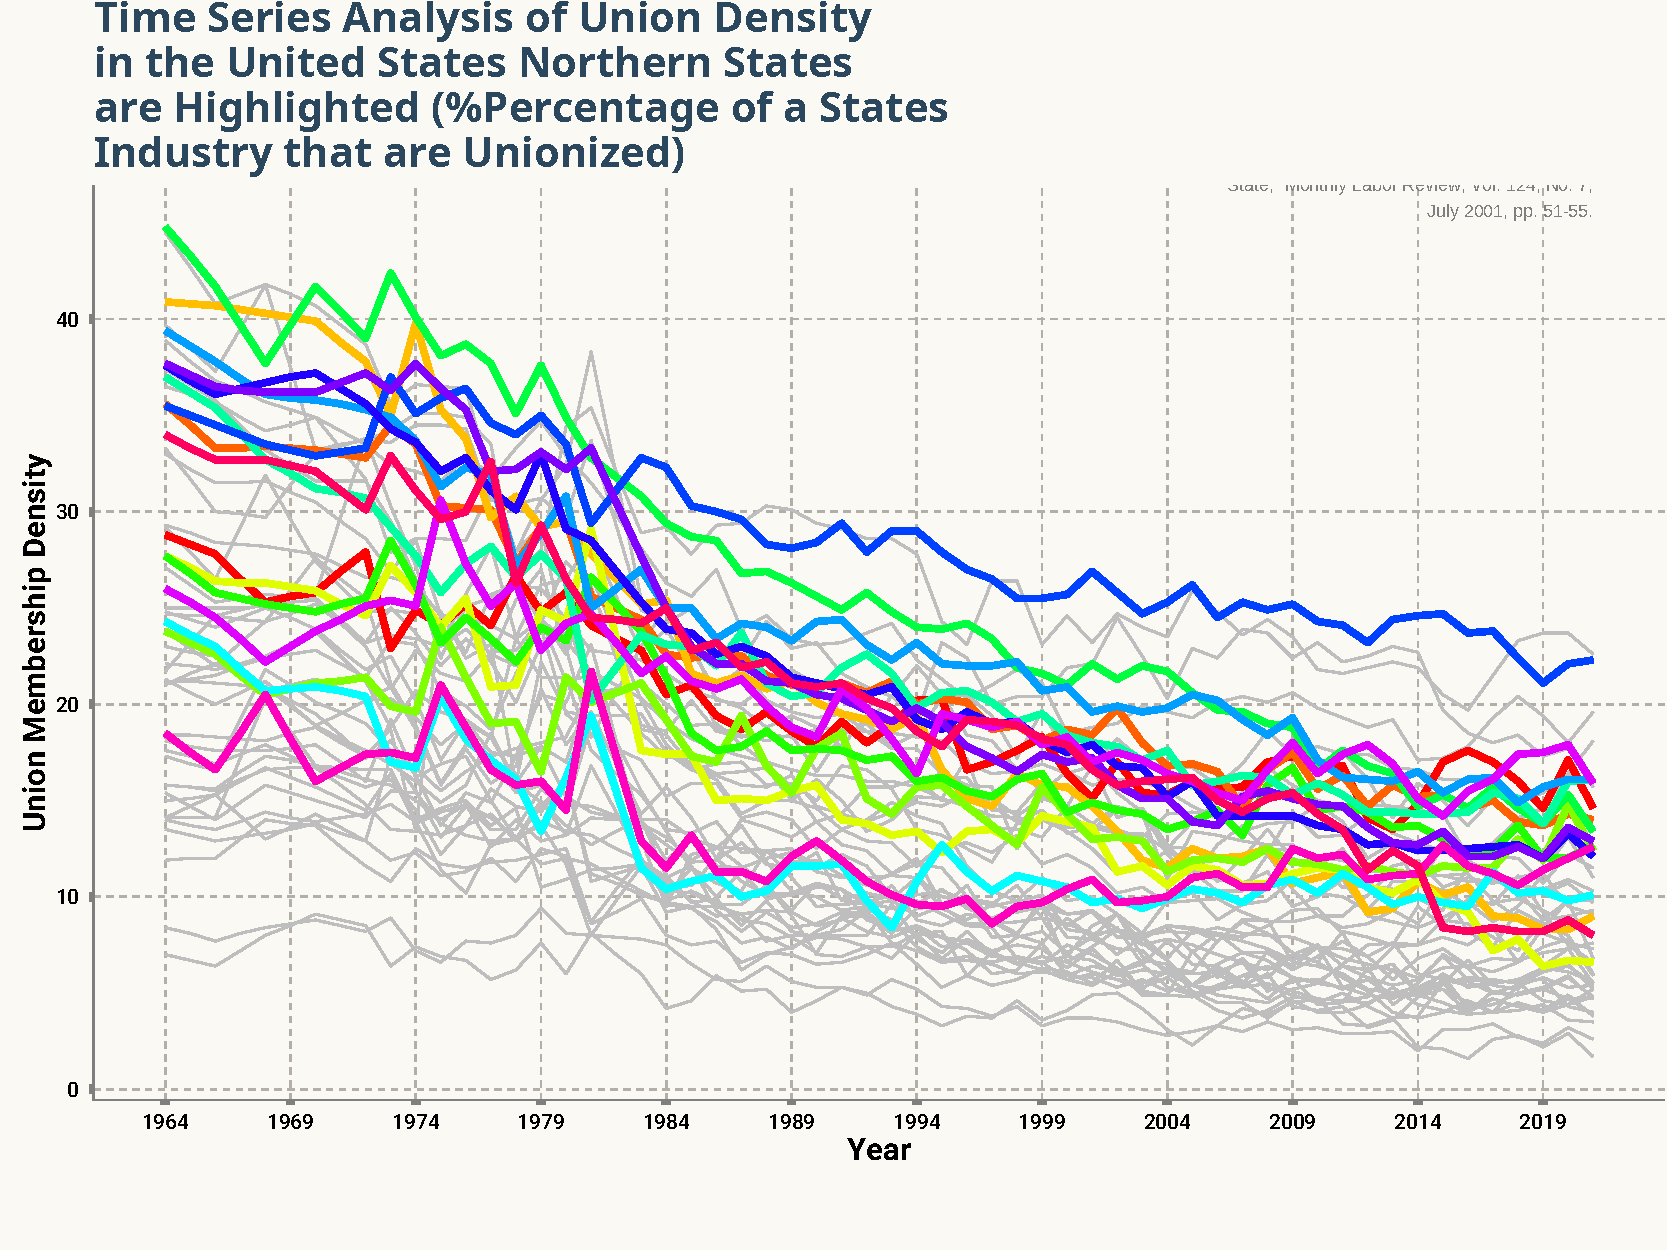
\includegraphics[width=.7\textwidth]{~/Lab2/graphs/plot_11.pdf}
\caption{[Detailed caption for Figure 2]}
\label{fig:1.2}
\end{figure}

\begin{figure}[h]
\centering
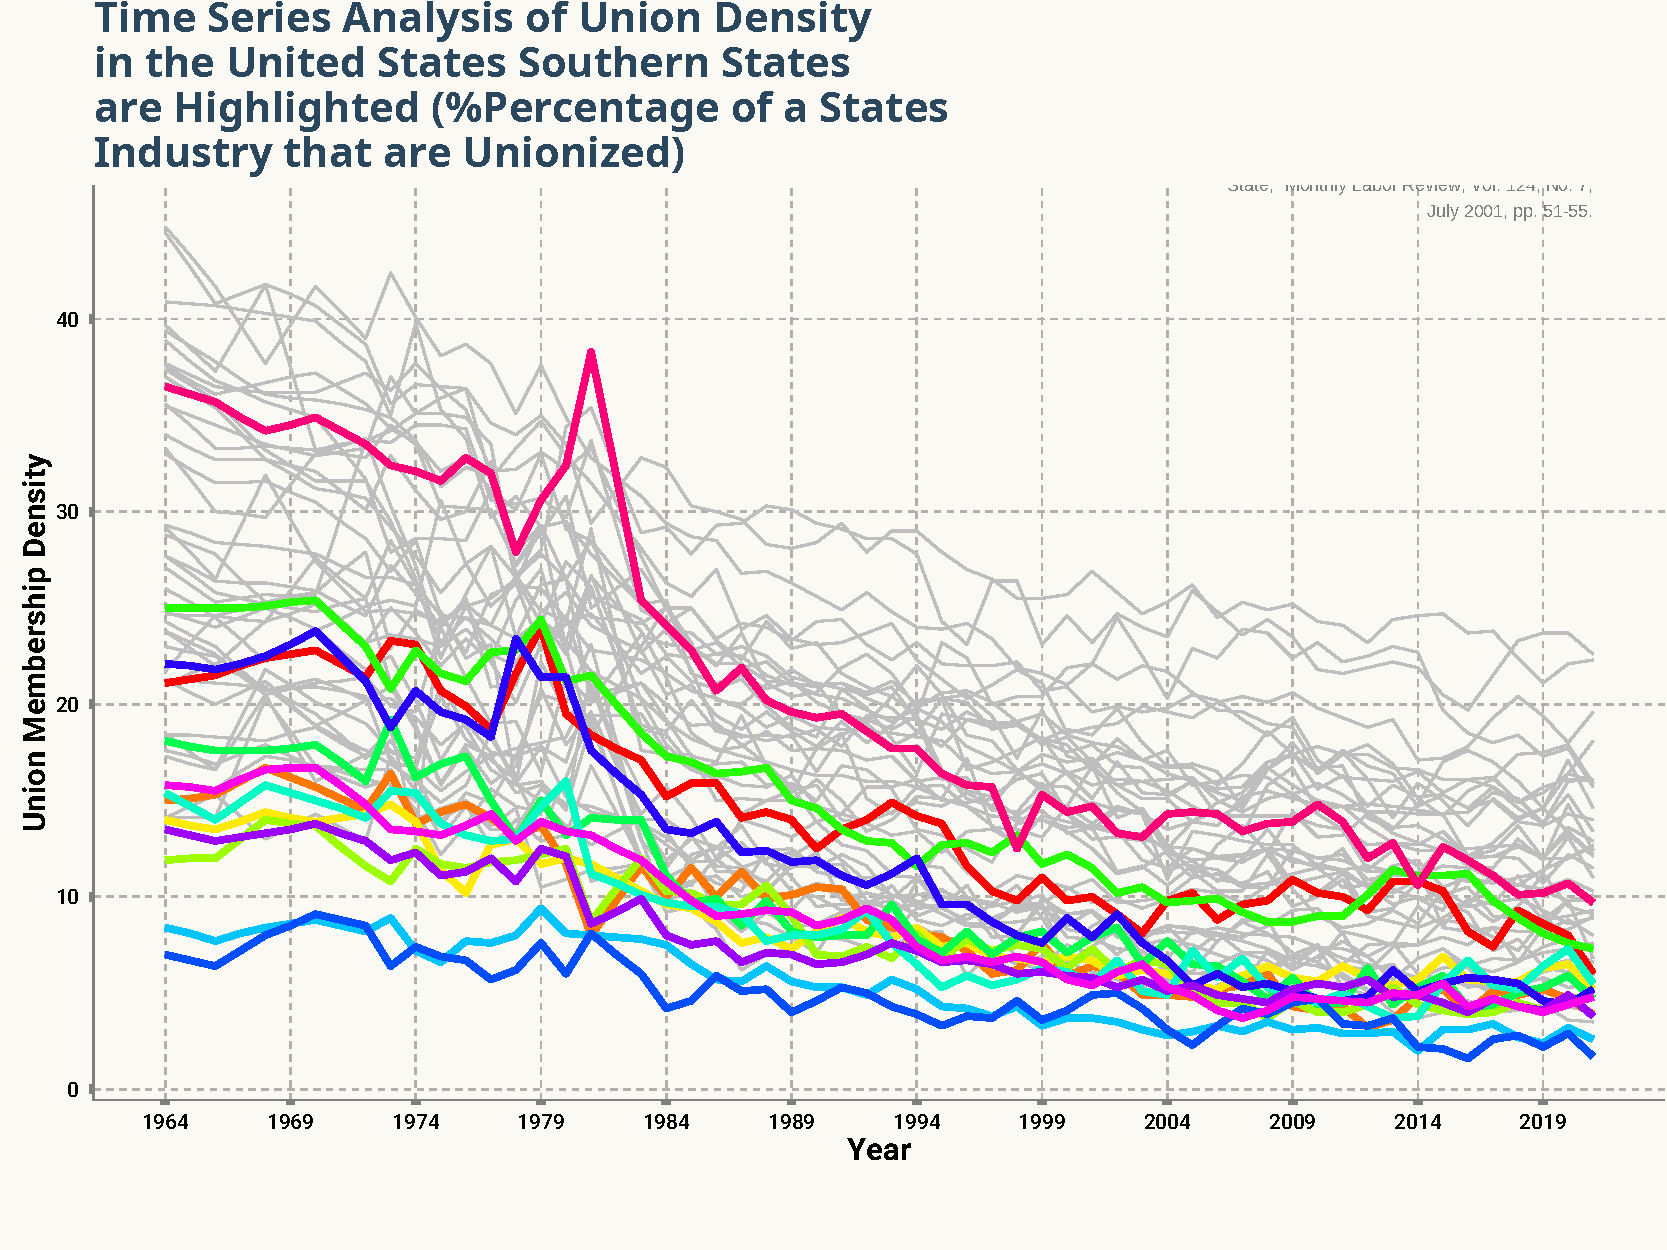
\includegraphics[width=.7\textwidth]{~/Lab2/graphs/plot_12.pdf}
\caption{[Detailed caption for Figure 3]}
\label{fig:1.3}
\end{figure}

\begin{figure}[h]
\centering
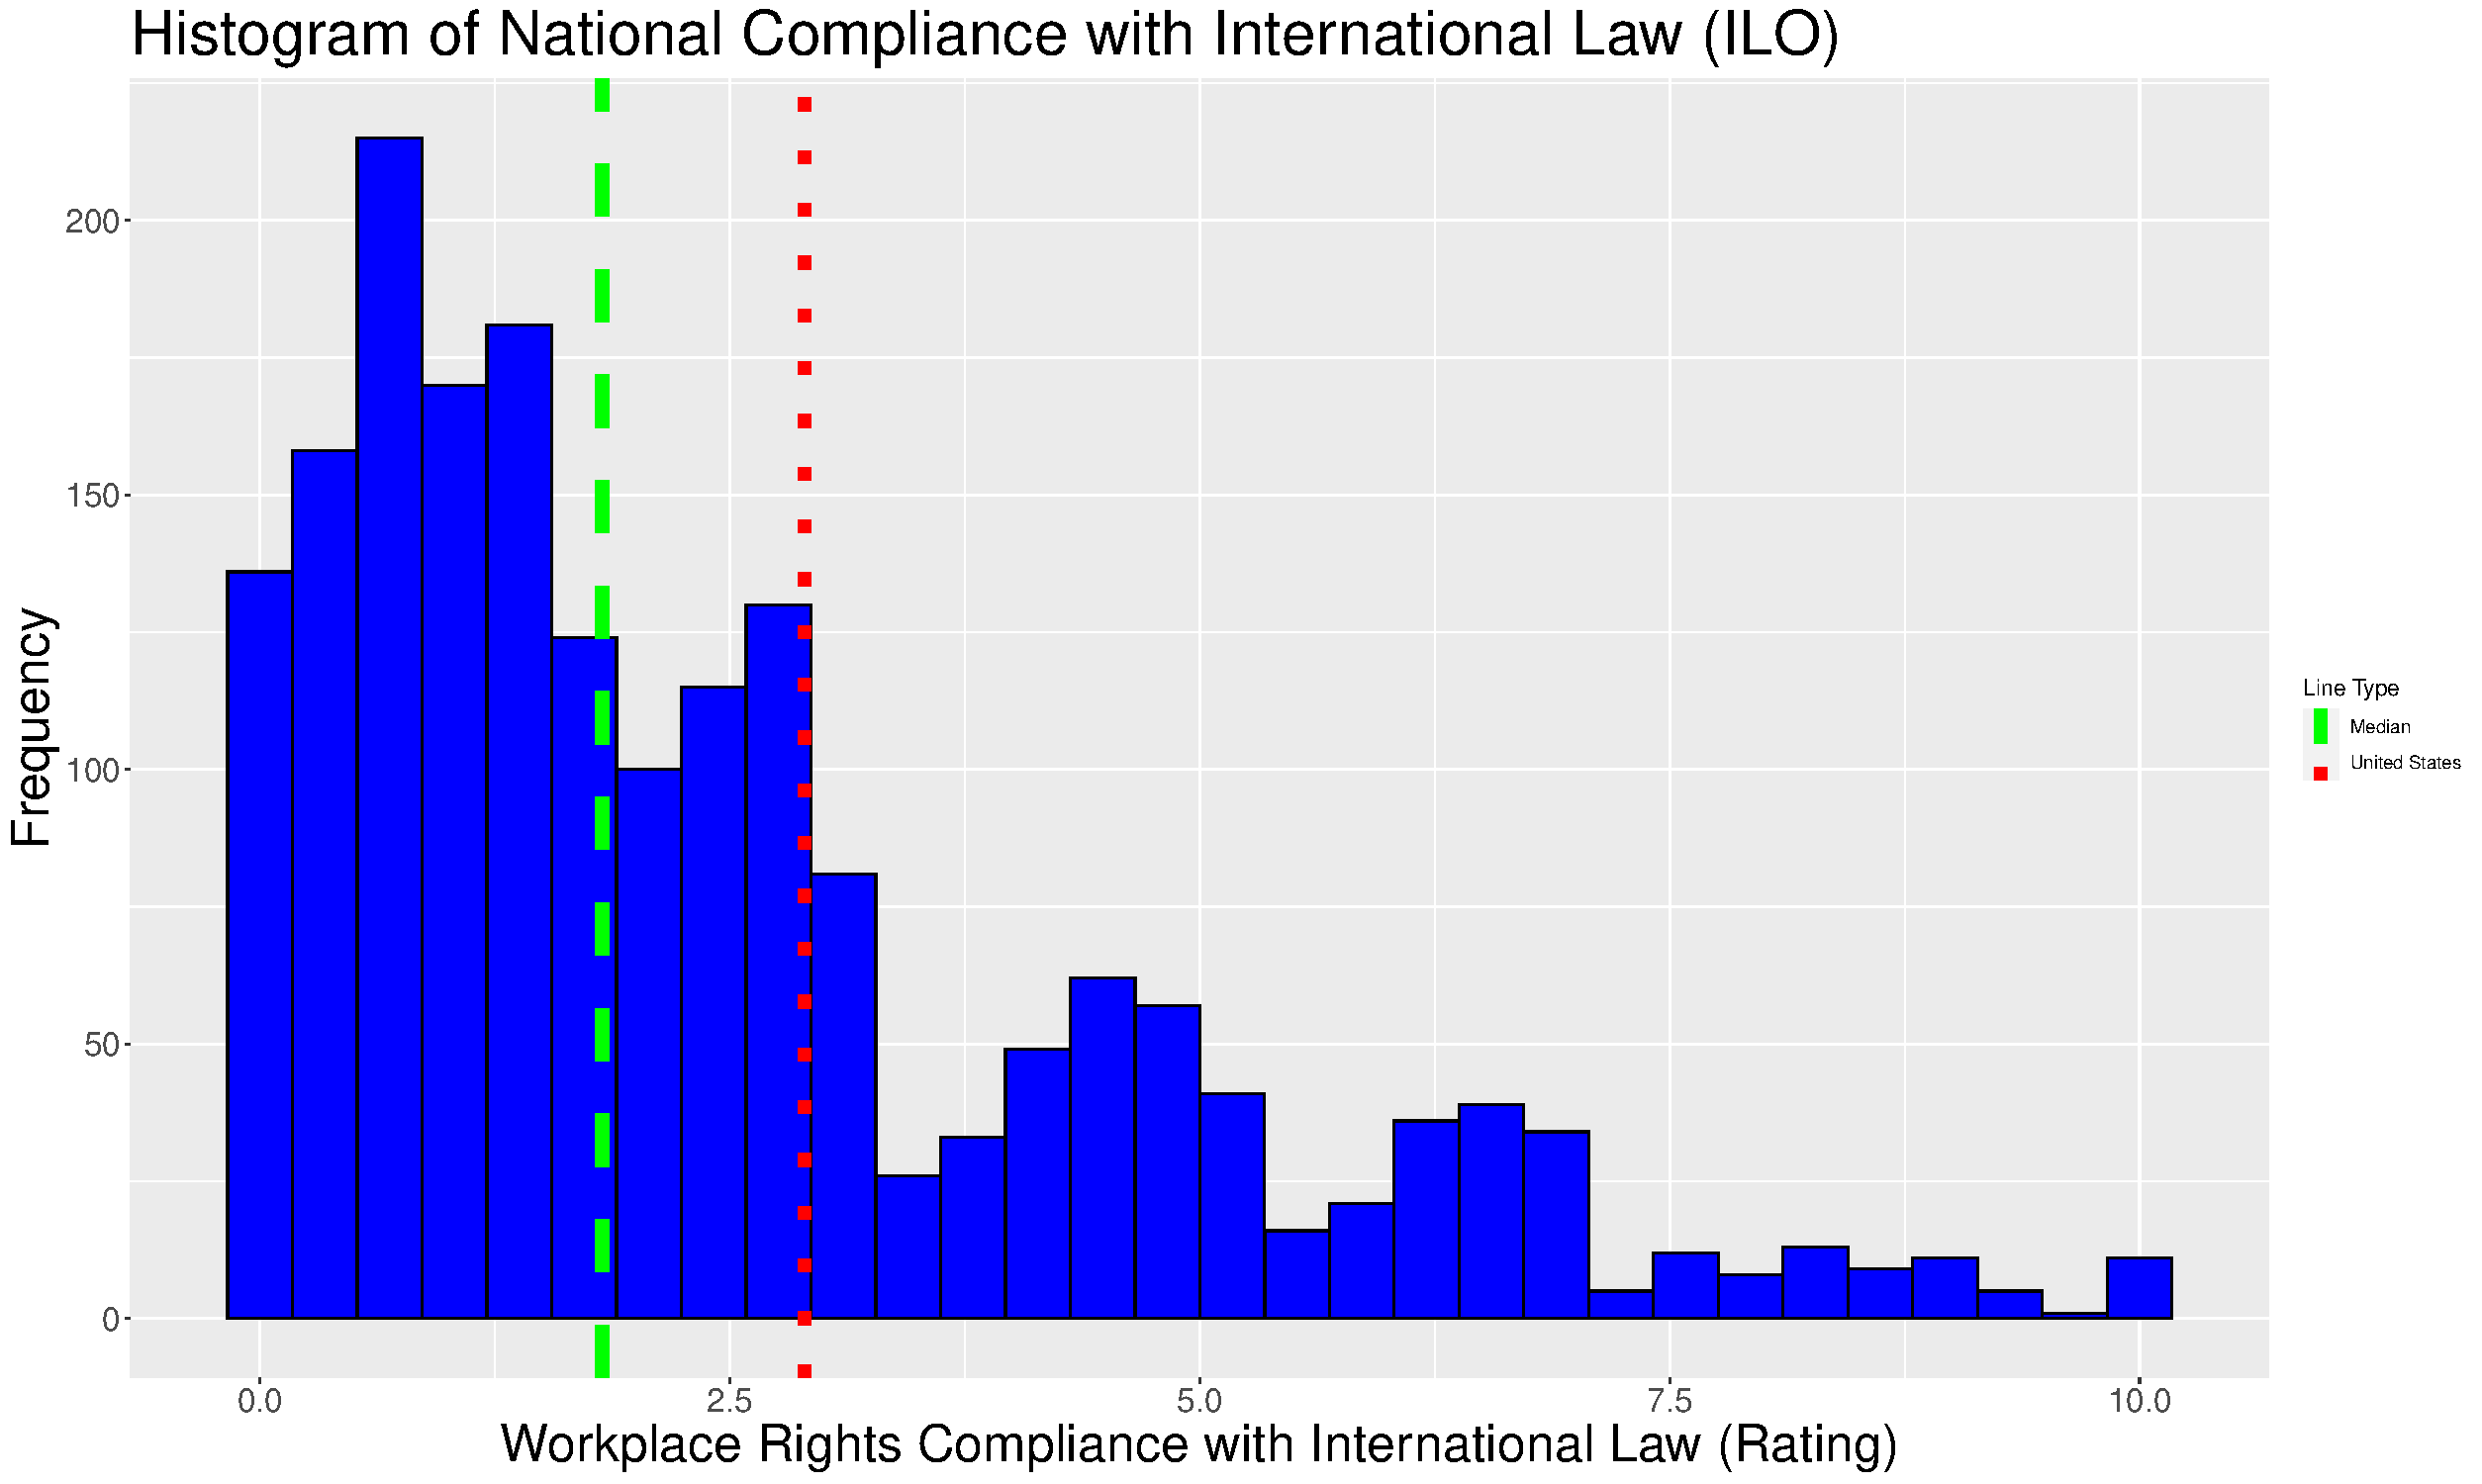
\includegraphics[width=.7\textwidth]{~/Lab2/graphs/plot_8.pdf}
\caption{Histogram depicting the frequency distribution of annual collective bargaining coverage measured in percent recorded by the International Labor Organization database. The data is grouped by country, highlighting the predominance of collective bargaining coverage in the United States compared to the rest of the world.}
\label{fig:2.1}
\end{figure}

\begin{figure}[h]
\centering
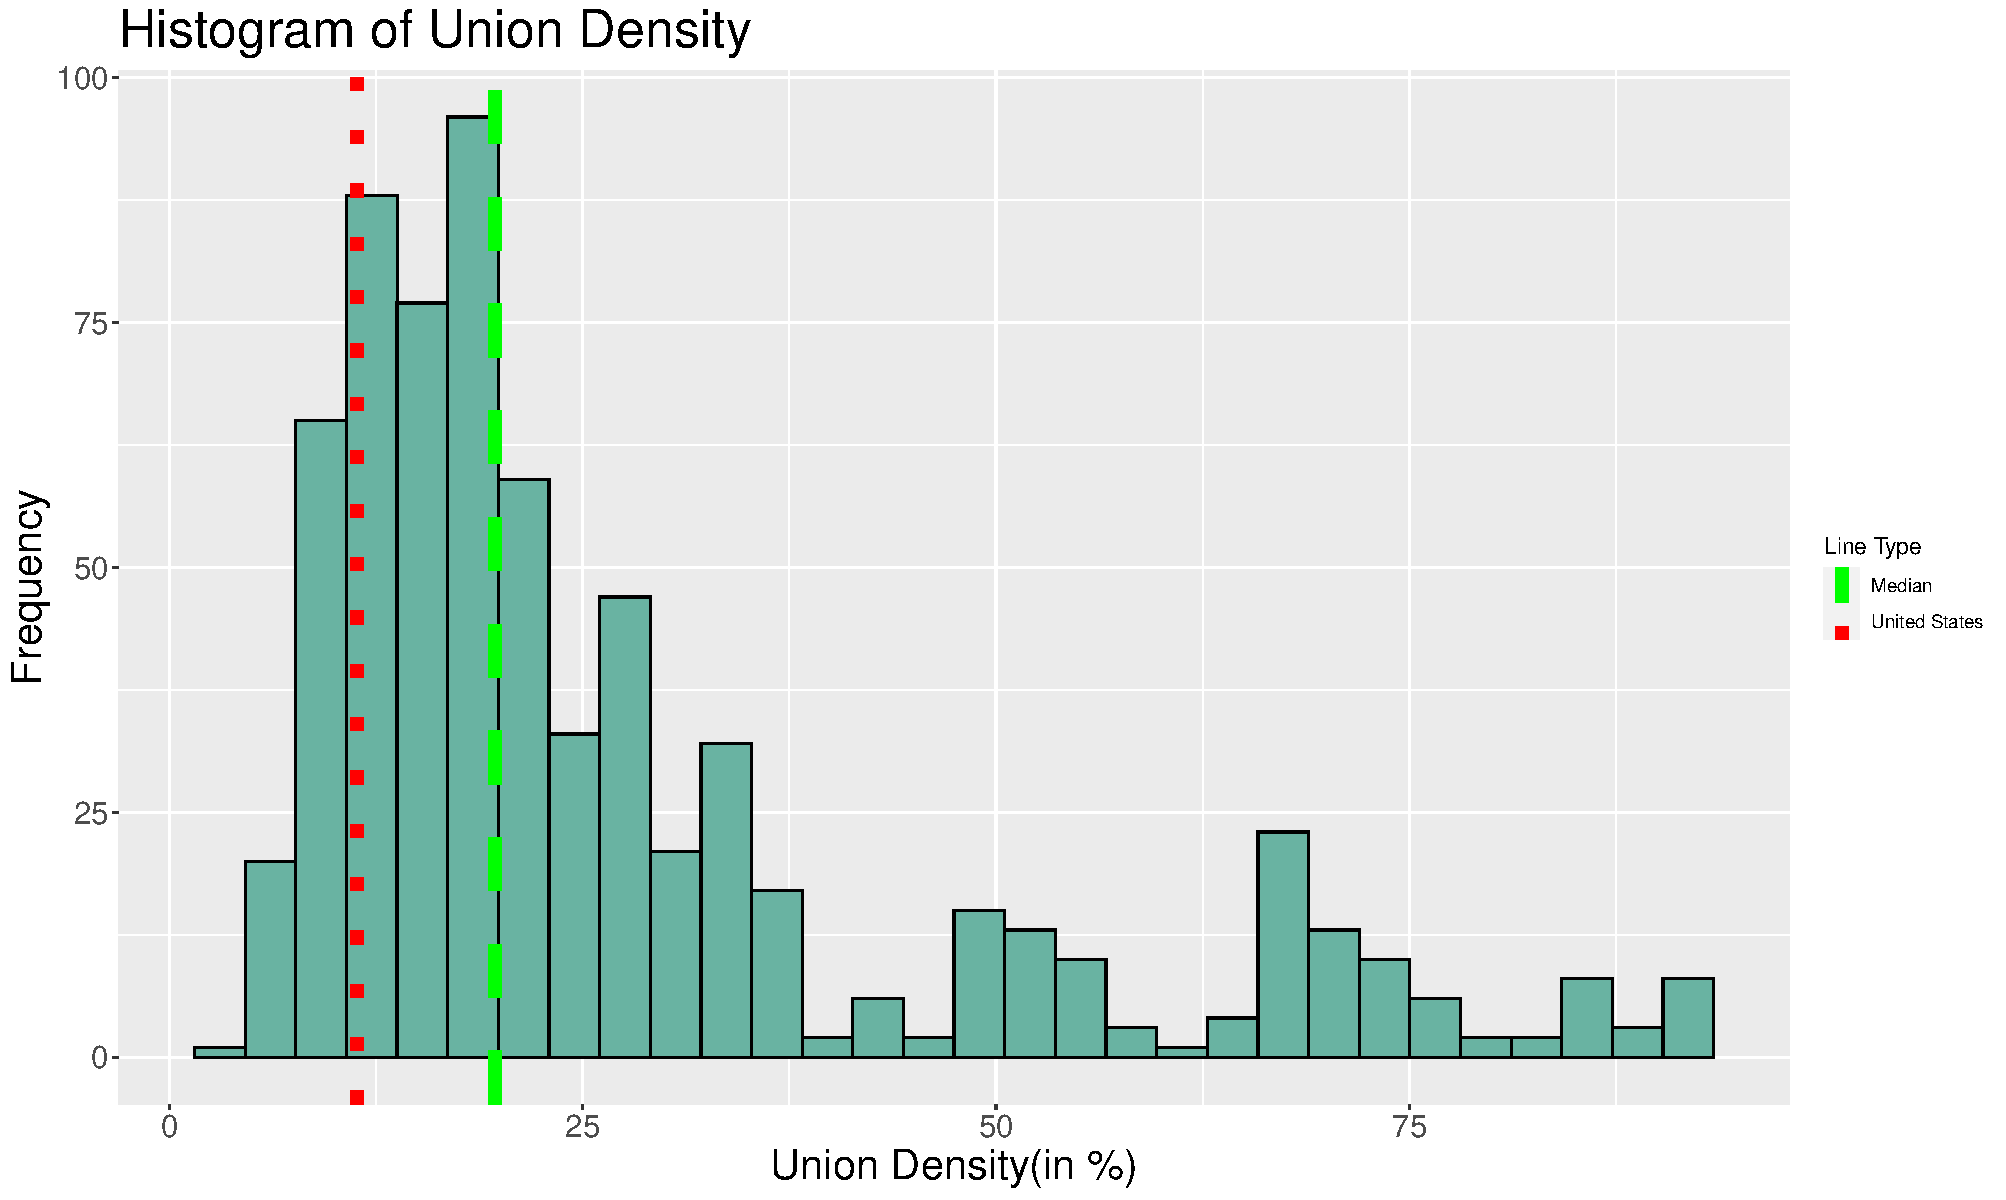
\includegraphics[width=.7\textwidth]{~/Lab2/graphs/plot_8-1.pdf}
\caption{[Detailed caption for Figure 5]}
\label{fig:2.2}
\end{figure}

\begin{figure}[h]
\centering
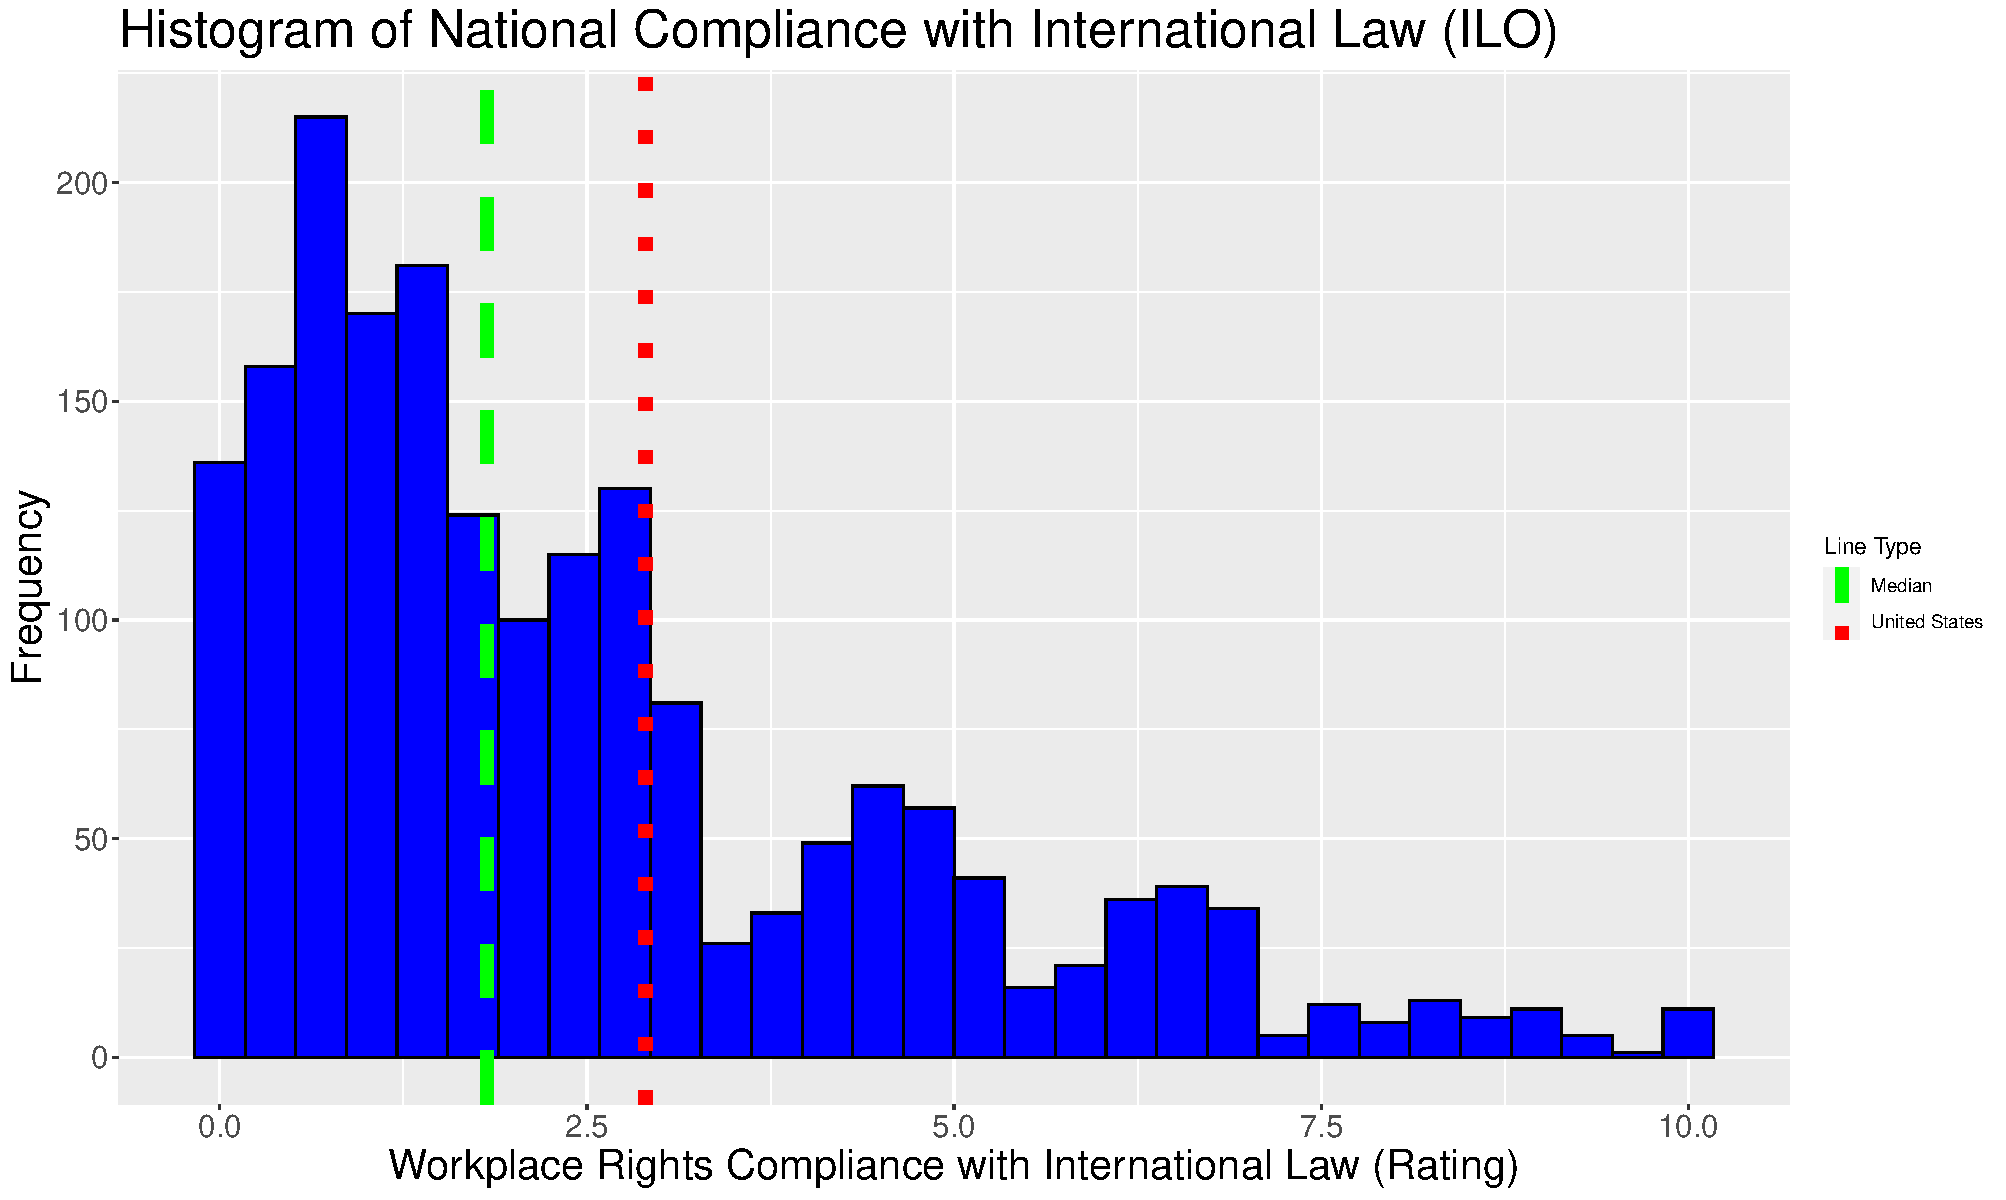
\includegraphics[width=.7\textwidth]{~/Lab2/graphs/plot_9.pdf}
\caption{Figure 2.3: Histogram depicting the frequency distribution of Compliance with international law bargaining coverage as scale from 0 to 10 with 10 being the most out of compliance with international law a country could be, and 0 being completely incompliance with international labor law recorded by the International Labor organization. This data is grouped by country, the united states place is marked in the along with the mean of all countries.}
\label{fig:2.3}
\end{figure}

\clearpage
\section{Conclusion}
Summarize the main findings and their relevance to the initial objectives of your study.


\clearpage
\section{References}
\begin{enumerate}
    \item Visser, J. (2021). OECD/AIAS database on Institutional Characteristics of Trade Unions, Wage Setting, 
      State Intervention and Social Pacts (ICTWSS) [Data set]. OECD. 
      Retrieved from 
      \url{https://www.oecd.org/employment/ictwss-database.htm}
    \item International Labour Organization. (2022). Trade union density rate () 
      -- Annual (Id: ILR\_TUMT\_NOC\_RT\_A) [Data set]. Industrial Relations Data (IRdata). 
      Retrieved from 
      \url{https://www.ilo.org/shinyapps/bulkexplorer30/?lang=en\&id=ILR\_TUMT\_NOC\_RT\_A}
    \item International Labour Organization. (2022). Collective bargaining coverage 
      rate () -- Annual (Id: ILR\_CBCT\_NOC\_RT\_A) [Data set]. 
      Industrial Relations Data (IRdata). Retrieved from 
      \url{https://www.ilo.org/shinyapps/bulkexplorer36/?lang=en\&id=ILR\_CBCT\_NOC\_RT\_A}
    \item International Labour Organization. (2023). SDG indicator 8.8.2 - 
      Level of national compliance with labour rights
      (freedom of association and collective bargaining) 
      based on ILO textual sources and national legislation -- 
      Annual (Id: SDG\_0882\_NOC\_RT\_A) [Data set]. 
      SDG Labour Market Indicators (ILOSDG). Retrieved 
      from \url{https://www.ilo.org/shinyapps/bulkexplorer30/?lang=en\&id=ILR\_TUMT\_NOC\_RT\_A}
\end{enumerate}


\end{document}
